\documentclass[a4paper,addpoints]{exam}

\usepackage[dvipsnames,table]{xcolor}
\usepackage{pgfplots}
\usetikzlibrary{decorations.markings}
\pgfplotsset{compat=1.8}
\usepackage{commath}
\usepackage{caption}
\usepackage{subcaption}
\usepackage{siunitx}
% russian integral
\usepackage{scalerel}
\DeclareMathOperator*{\rint}{\scalerel*{\rotatebox{17}{$\!\int\!$}}{\int}}
\qformat{\textbf{\large{Question \thequestion: \thequestiontitle}}\hfill}
\pointsinrightmargin

\begin{document}

\begin{coverpages}

\begin{center}
  
\includegraphics[width=0.6\textwidth]{edyn_cover}

  \vspace{5mm}

  \textbf{\Huge{Level Two Physics: Electrodynamics}}
\end{center}

\vspace{5mm}

\noindent
\large{There are three questions, worth a total of \numpoints\ marks.\\
       Attempt ALL questions, showing all working.\\
       Read questions carefully before attempting them.\\
       Marks are available for partial answers.\\
       The amount of time expected to be spent per question may not necessarily correlate ``nicely'' to the number of marks.\\
       Diagrams may be used to support answers.\\
       Candidates who do not provide diagrams for some questions may be disadvantaged.\\
       Some marks are given for clarity and neatness of solutions or proofs.}
\vspace{2mm}

\vfill

\begin{flushright}
  \begin{tabular}{ll}
    \textbf{Time Allowed:}& One Hour\\
    \textbf{Achieved:}& 9 marks\\
    \textbf{Merit:}& 14 marks\\
    \textbf{Excellence:}& 20 marks
  \end{tabular}

  \gradetable[v][questions]
\end{flushright}

\end{coverpages}

\begin{questions}
  \titledquestion{Fun with Circuits}
    Consider the following circuit.
    \begin{center}
      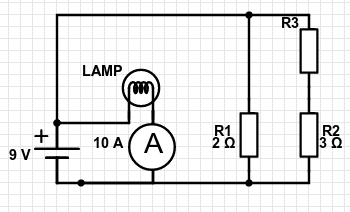
\includegraphics[width=0.4\textwidth]{circuit1}
    \end{center}
    \begin{parts}
      \part[1] Find the resistance of the light bulb.
      \part[4] Calculate the value of $ R_3 $.
      \part[3] Explain why the lamp dissipates more power than $ R_3 $.
    \end{parts}
  \titledquestion{Fun with Particles}
    A positively charged particle enters a perpendicular magnetic field (of magnitude \SI{1}{\tesla}) as shown.
    \begin{center}
      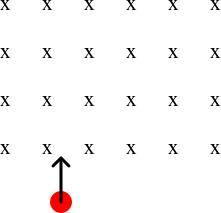
\includegraphics[width=0.2\textwidth]{magf1}
    \end{center}
    \begin{parts}
      \part[4] Describe and comprehensively explain the shape and direction of the path followed by the particle.

            \textit{You may wish to:}
            \begin{itemize}
              \item Describe the force(s) acting on the particle in the field.
              \item Describe the acceleration(s) felt by the particle.
              \item Explain the resulting change(s) in velocity of the particle.
            \end{itemize}
            \textit{Candidates may include a diagram in their answer.}
      \part[1] The force felt by the particle is initially measured to be \SI{0.10}{\newton}, and it is
            moving with a speed of \SI{3.00}{\metre\per\second}. Calculate the magnitude of the particle's charge.
      \part[3] The particle has a mass of \SI{1.23}{\micro\gram} ($ \SI{1}{\micro\gram} \equiv \SI{1e-6}{\gram} $). How much
            work is done on the particle by the magnetic field over the first three seconds that it is in the magnetic field?
            Explain your answer.
    \end{parts}
  \titledquestion{Fun with Wires in Magnetic Fields}
    A straight conductor is carring a current of magnitude \SI{3.0}{\ampere}. Suddenly, a perpendicular magnetic field is produced around a
    section of the conductor that is \SI{2.0}{\metre} long. This section has a total resistance of \SI{10}{\ohm}.
    \begin{parts}
      \part[3] Explain why the conductor is observed to move.
      \part[2] The magnitude of the electric field is $ B = \SI{0.53}{\tesla} $. Compute the magnitude of the initial
            induced force on the wire.
      \part[3] Explain, with reference to the laws of Faraday and Lenz, why the force felt by the wire diminishes over time.
    \end{parts}
\end{questions}

\end{document}
